
In this section, we provide some background that will be used later. We first introduce several mathematical concepts that will be used in the second part, where we describe homology, which is essential for introducing the methods in subsequent sections.


\subsection{A Crash Course on Topology} \label{sec:topology}

Topology, a core discipline in mathematics, studies the properties of shapes and spaces that remain unchanged under continuous transformations such as stretching, crumpling, and bending, but not tearing or gluing. In machine learning, topology provides a powerful framework for examining complex data structures flexibly and intuitively. To provide clarity, we begin by defining several key terms essential for following the paper.

\subsubsection{Topological Space} From a mathematical perspective, topology refers to \textit{the structure of a set}. For instance, consider the set of real numbers between $0$ and $1$, i.e., $\X = \{x\in\R \mid 0 \leq x \leq 1\}$. Many readers might immediately consider the closed interval $[0,1]$, whose shape resembles a stick. However, $\X$ is merely a set with no defined structure yet. This means we do not know which points in $\X$ are close to or far from others, as there is no concept of neighborhoods.

For example, if we define a distance (metric) on $\X$ such as $d_1(x, y) = 1$ for $x \neq y$ and $d_1(x, y) = 0$ for $x = y$, the "shape" of the set $\X$ would be entirely different, resembling an infinite number of points dispersed in a very high-dimensional space. Conversely, if we use a metric like $d_2(x, y) = |x - y|$ on $\X$, we retrieve our familiar closed interval $[0,1]$, a stick of length $1$. Notice that due to the different metrics used, the neighborhood structures and shapes of $(\X, d_1)$ and $(\X, d_2)$ are completely different. This brings us to the first principle in Topology: \textit{the topology of a set} is defined as the complete neighborhood information on the set.  

The principle is not without exceptions: a significant research area called \textit{point-set topology} studying topological spaces that do not necessarily have a metric~\cite{lopez2024point,goubault2013non}. However, these topologies are beyond our scope. Thus, throughout the paper, a \textit{topological space} refers to a set $\X$ (or dataset) equipped with a distance $d(\cdot,\cdot)$, forming what is known as a \textit{metric space} $(\X,d)$. In other words, a set qualifies as a topological space if we can unambiguously identify the neighbors of its points. 



Although we might not explicitly reference distance, most datasets inherently possess some form of a metric for detailed analysis. For instance, point clouds use the metric of the space they are embedded in, providing neighboring information. In graphs, adjacent nodes are naturally considered neighbors. Similarly, in images, neighboring pixels are deemed neighbors. This paper treats these examples as topological spaces with their natural topologies. However, specific datasets, such as RNA-sequencing data, lack an inherent metric, requiring users to define a metric to determine which data points are considered close and distant, depending on the context.

\paragraph*{Simplicial Complexes.} One special family of topological spaces used throughout our paper will be {\em simplicial complexes.} A simplicial complex is a mathematical structure used in topology and combinatorics to study the properties of shapes and spaces in a \textit{discrete manner}. It consists of vertices, edges, and higher-dimensional simplices such as triangles, tetrahedra, and their higher-dimensional counterparts, which are glued together in a specific way to form a coherent whole. 



Each simplex is a generalization of the concept of a triangle to higher dimensions. By this, we mean that the properties and structure of a triangle (such as having vertices, edges, and faces) are extended into higher dimensions, even though the shapes look different as we go up in dimensions. In particular, a $k$-simplex is defined as the convex hull of affinely independent $k+1$ points in $\R^k$. For example, $2$-simplex is a triangle (with its inside filled), e.g., the convex hull of (smallest convex set containing) three points $\{(0,0), (1,0),(0,1)\}$ in $\R^2$. Similarly, $3$-simplex is a tetrahedron (with inside filled), e.g., the convex hull of $\{(0,0,0), (1,0,0),(0,1,0),(0,0,1)\}$ in $\R^3$. A union of simplices is called a \textit{simplicial complex} if any two simplices in the complex either do not intersect or intersect in a complete subsimplex (See \Cref{fig:scsample}).


\begin{wrapfigure}{r}{3in}
\vspace{-.2in}
    \centering
    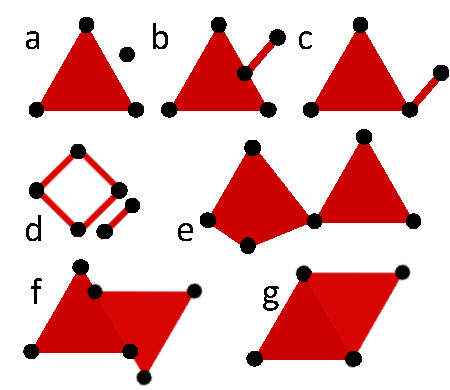
\includegraphics[width=\linewidth]{figures/scsamples.pdf}
        \caption{\textbf{Simplicial Complexes.} Among the complexes, only b and f fail to be simplicial complexes, as their simplices do not intersect at complete subsimplices. All others are valid simplicial complexes. \label{fig:scsample}}
    \vspace{-.2in}
\end{wrapfigure}

\paragraph*{Dimension in Topology} One of the most confusing concepts for non-experts in topology is the notion of dimension. To study topological spaces more effectively, we focus on a specific family of spaces that meet certain regularity conditions, known as \textit{manifolds}. A $k$-dimensional manifold is a topological space that locally resembles a ball in $\R^k$, i.e., a small neighborhood of any point looks like (homeomorphic) a ball in $\R^k$. 
Importantly, we do not concern ourselves with the ambient (i.e., surrounding) space in which our manifold resides; we focus solely on its intrinsic properties, e.g., \textit{the material the manifold is made of}. For example, although a circle is often visualized in $\R^2$ as a two-dimensional object, from a topological perspective, it is actually one-dimensional. This is because, at any point on the circle, its local neighborhood resembles a line segment, i.e., it is made of $1$-dimensional material. Consider an ant walking on a circle; it has two options: moving forward or backward. While we might need two coordinates to describe the ant's position on the circle mathematically, from the ant's perspective, it only experiences a continuous path where it can move in either direction. To the ant, the circle feels like an endless line. Similarly, a sphere is a $2$-dimensional manifold (surface) even though it is often visualized in $\R^3$. This is because a small neighborhood of any point on the sphere resembles a piece of in $\R^2$. Notice that with this definition, the dimension of the ambient space becomes irrelevant; only the topological properties define the dimension of a manifold, i.e., a loop (circle) in $\R^2$  or $\R^3$ is called $1$-dimensional.  Similarly, a torus (a hollow donut) and a genus-2 surface (a surface with two holes) are examples of 2-dimensional manifolds. If this discussion leads you to wonder about manifolds with more than two dimensions, we have some discouraging news: they do exist, but visualizing them is not intuitive.



\paragraph*{Boundary.} In topology, understanding the boundary of a manifold is crucial to grasping its structure. A $k$-dimensional manifold $M$ is a space where each point has a neighborhood that resembles an open subset of $\R^k$. The boundary $\partial M$ of $M$ comprises points where these neighborhoods resemble an open subset of the half-space $\R^k_+ = \{ x \in \R^k \mid x_k \geq 0 \}$. This implies that the local structure is similar to part of $\R^k_+$ near each boundary point.

To illustrate, consider a sphere, a 2-dimensional surface without any boundaries. An ant walking on the sphere can indefinitely move in any direction without encountering an edge. In contrast, the unit disk $\D$ in $\mathbb{R}^2$ is a 2-dimensional surface with a boundary, specifically the unit circle $\C$.  An ant residing in $\D$ could not continue its journey once it reaches the boundary $\C$, or the "border" of $\D$. This is denoted as $\partial \D = \C$. Similarly, the unit ball $\B$ in $\R^3$   (the solid ball) is a 3-dimensional manifold with a boundary, and its boundary is the unit sphere $\s$, denoted by $\partial \B = \s$. In this context, we say that the sphere $\s$ bounds the ball $\B$.

If you're puzzled by the statement that \textit{ a sphere has no boundary, whereas the solid ball does}, consider it from the perspective of "its inhabitants." An ant living on the sphere's surface can move freely in any direction without ever encountering a limit (no border), which is why we say the sphere has no boundary. However, a mouse living inside the ball will eventually hit the boundary (border)—the sphere's surface—beyond which it cannot go. That limiting surface is what we call the solid ball's boundary. 
%\textN{The fact that sphere does not have but ball has a boundary is confusing. To CS they are the same}\BC{Figures}

A key principle in topology is that a boundary's boundary is always empty. Mathematically, this is expressed as $\partial (\partial \X) = \emptyset$. Furthermore, the boundary of a $k$-dimensional manifold is generally a $(k-1)$-dimensional manifold with no boundary. For example, the boundary of a disk $\D$ (a 2-dimensional manifold with a boundary) is a circle $\C$ (a 1-dimensional manifold without a boundary). This observation will soon be important when discussing homology. 


\subsubsection{Topological Equivalence} Topology primarily focuses on the global properties of shapes rather than their local characteristics. For example, topology is concerned with whether a space is connected or has holes without regard to the size of the object or the holes. 

Topological equivalence can be intuitively understood as follows: two shapes, $\X$ and $\Y$ are topologically equivalent if one can be continuously deformed into the other. Imagine $\X$ and $\Y$ are made of Play-Doh. If you can reshape $\X$ into $\Y$ without tearing, gluing, or collapsing any part of the shape, then they are considered to be continuously deformable into each other.  In this context, "collapsing" refers to reducing a part of the shape to a lower dimension, such as squishing a surface or line down to a point or flattening a 3-dimensional object into a 2-dimensional plane.

In mathematical terms, this concept corresponds to a \textit{homeomorphism} (the prefix "homeo-" comes from the Greek word "homoios," which means "similar" or "like"). In particular, such a deformation from $\X$ to $\Y$ represents a bijective map, which means it creates a one-to-one correspondence between elements of $\X$ and $\Y$, ensuring that each element in $\X$ is paired with a unique element in $\Y$ and vice versa. The map $\varphi:\X \to\Y$ keeps track of how each point $x \in\X$ becomes a point $y \in\Y$ after the deformation, i.e., $\varphi(\X) = y$. The condition of no tearing ensures that this map is continuous as nearby points in $\X$ must map to nearby points in $\Y$. Gluing is the opposite of tearing, so we also require that the inverse map $\varphi^{-1}$ is continuous. In summary, $\varphi:\X \to\Y$ is called a \textit{homeomorphism} if $\varphi$ is a continuous bijection with a continuous inverse.

We previously noted that size does not affect the topological structure. For example, let $\X = \R$, the set of all real numbers, and $\Y = (-1, 1)$, the open interval containing all real numbers between $-1$ and $1$, excluding the endpoints. These two spaces are topologically equivalent via the homomorphism $\varphi:\R\to(-1,1)$ with  $\varphi(x) = \frac{x}{1 + |x|}$. However, $\R$ has an infinite diameter, while $(-1,1)$ has a diameter of only 2. Hence, this is a good example of how the space size does not matter in topology. On the other hand, consider $\X = (0,1) \cup (1,2)$ and $\Y = (0,2)$. While both spaces are similar as sets, they are not topologically equivalent because $\X$ consists of two separate connected components, whereas $\Y$ is a single connected piece. A continuous deformation (homeomorphism) must preserve the number of components.

 
\paragraph*{Homotopy.} Another important concept in topology is {\em homotopy}, which can be seen as a flexible deformation of one space into another. Unlike homeomorphism, homotopy allows for collapsing but not tearing or gluing. We call two spaces homotopic to each other if such a deformation exists from one to another. For instance, a disk and a point are homotopic because the entire disk can be collapsed into a point by pushing inwards from all directions towards the center. Similarly, a punctured disk ($\mathbf{D}^2-\{(0,0)\}$) and a circle are homotopic, as a punctured disk can be continuously deformed towards its boundary, starting from the puncture point $(0,0)$. Homotopy provides a powerful tool for classifying topological spaces and understanding their fundamental properties, as most topological invariants are homotopy invariants, meaning they yield the same output for two homotopic spaces. For example, the connectivity and the count of holes or cavities do not change under homotopy.



\subsubsection{Topological Invariant} \label{sec:top_invariant} If  two spaces $\X$ and $\Y$ are topologically equivalent, showing that there is a homeomorphism $\varphi: \X \to \Y$ would be sufficient. However, if they are topologically different, one must demonstrate that no such map can exist, which is highly challenging. Mathematicians use invariants to show such inequivalence. An invariant refers to a property or feature of an object that remains unchanged under certain transformations. A \textit{topological invariant} is an invariant that is preserved under homeomorphism. A topological invariant can be a number (number of components, Euler characteristics, Betti numbers), a mathematical object (homology groups, fundamental group, cohomology ring), or a mathematical property (compactness, connectedness). 



\begin{wrapfigure}{r}{3in}
\vspace{-.2in}
    \centering
    \subfloat[Sphere]{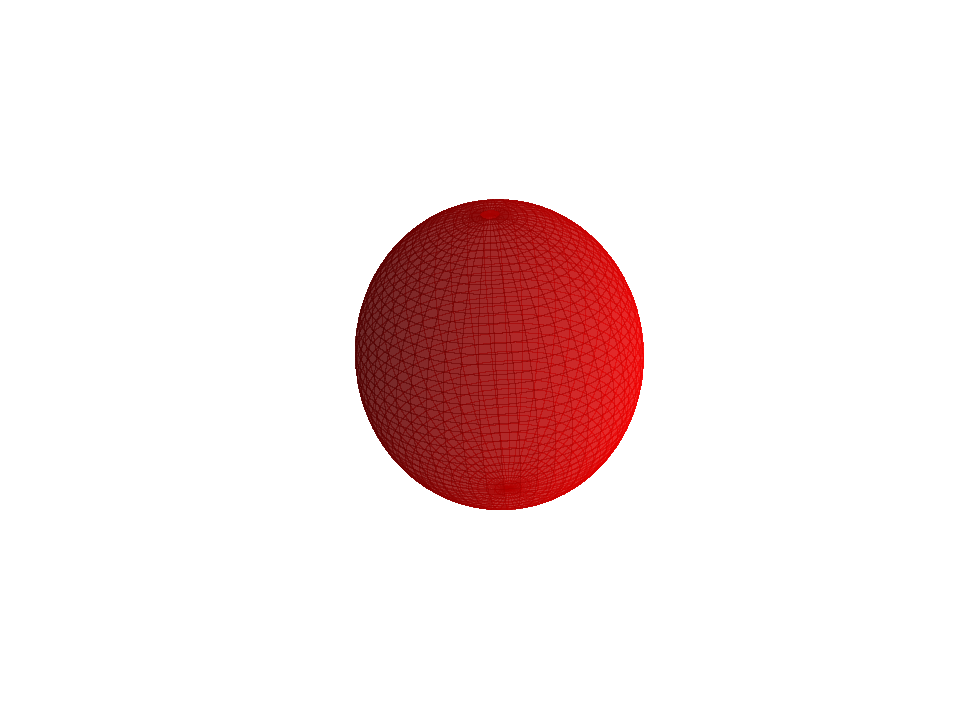
\includegraphics[width=0.3\linewidth]{figures/sphere.pdf}\label{fig:sphere}}
    \subfloat[Cube]{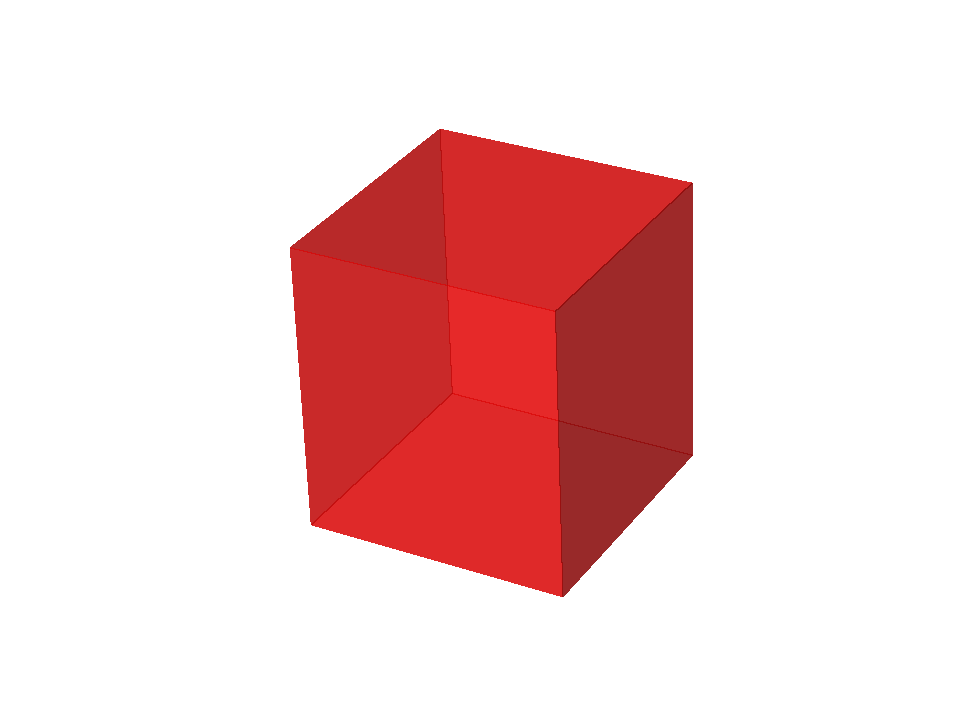
\includegraphics[width=0.3\linewidth]{figures/cube.pdf}\label{fig:cube}}
    \subfloat[Torus]{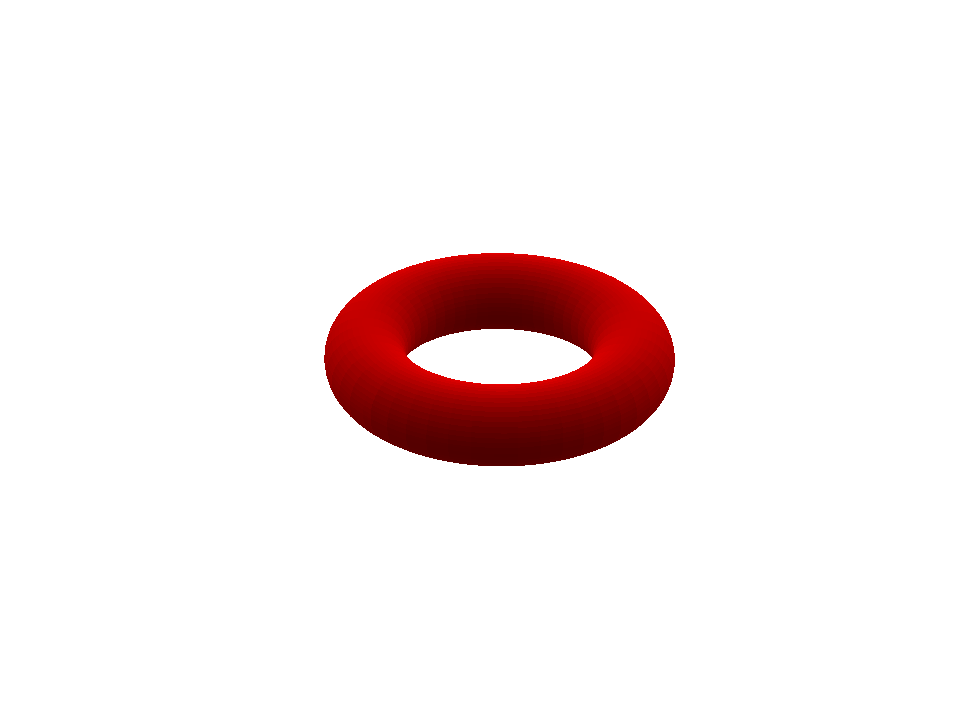
\includegraphics[width=0.3\linewidth]{figures/torus.pdf}\label{fig:torus}}
    \caption{The sphere and the cube are topologically equivalent, whereas the torus is different from both.}
    \label{fig:sphere_and_torus}
    \vspace{-.1in}
\end{wrapfigure}

In the example above, $\X = (0,1) \cup (1,2)$ versus $\Y = (0,2)$, we used the number of components as a topological invariant to show they are not equivalent. However, more subtle examples require more sophisticated invariants. For instance, a cube and a sphere are topologically equivalent because one can deform a cube into a sphere without tearing or gluing. In contrast, comparing a sphere and a torus (the surface of a donut as shown in ~\ref{fig:torus}) is more complex. They are not topologically equivalent because the torus has "holes." By holes, we mean the loops on the surface, which cannot be shrunk down to a point \textit{without leaving the surface}. From this perspective, a sphere has no hole, however, on a torus, some loops (meridian and longitude) can't be shrunk down to a point in the torus, representing the "holes" in torus (see \Cref{fig:homology}). Despite this difference, proving that a sphere and a torus are not homeomorphic is challenging. Therefore, subtle topological invariants that detect these holes are crucial for distinguishing such spaces. 

\paragraph*{Euler Characteristics} One important and well-known example of such topological invariants is the {\em Euler characteristic}. If $\C$ is a simplicial complex, we define the Euler characteristic as the alternating sum of the count of $k$-simplices in $\C$, i.e., $\chi(\C) = \sum_k (-1)^k n_k$, where $n_k$ is the count of $k$-simplices in $\C$. It turns out the Euler characteristic is a topological invariant. i.e., if $\C$ and $\D$ are homeomorphic, then $\chi(\C) = \chi(\D)$. The Euler characteristic is, in fact, a homotopy invariant as well (see \cite{hatcher2002algebraic}). For example, a sphere $\s$ is topologically equivalent to the surface of a hollow tetrahedron $\F$, which has 4 vertices ($n_0$), 6 edges ($n_1$), and 4 triangles ($n_2$). Therefore, we have $\chi(\s) = \chi(\F) = n_0 - n_1 + n_2 = 4 - 6 + 4 = 2$. Similarly, if one computes the Euler characteristic of a torus $\T$ through a simplicial complex, we find that $\chi(\T) = 0$. Since $\chi(\s) \neq \chi(\T)$, it follows that a sphere is not homeomorphic to a torus.

 

\subsubsection{Geometry vs. Topology} Before proceeding, let's clarify a common confusion between the terms \textit{topology} and \textit{geometry}. Both are branches of mathematics, but they focus on different aspects of metric spaces.

Geometry focuses on the \textit{local study} of shapes, sizes, and properties of space, as well as how these spaces embed (fit into) higher-dimensional spaces.  For example, a 2-dimensional sphere $\s$ can be embedded into $\R^3$ (or $\R^{10}$) in various shapes and sizes.
Geometry focuses on precise measurements (e.g., angles, distances, curvature) and the relationships between points, lines, surfaces, and solids. It explores how shapes bend and twist, providing tools to understand complex surfaces and spaces through concepts such as curvature and geodesics (i.e., shortest paths).

In contrast, topology examines the \textit{global properties} of space that remain unchanged under continuous deformations. It focuses on qualitative aspects like connectedness and continuity rather than precise measurements. For instance, topology considers a cube and a sphere as topologically equivalent because these shapes can be transformed into one another through continuous deformation despite their geometric differences—one being flat and the other curved. For instance, no matter how we embed a 2-sphere into $\mathbb{R}^{10}$, its topological properties remain unchanged. However, the geometry varies significantly: a round sphere with a radius of 1 differs greatly from one with a radius of 100. Moreover, an irregular sphere would be geometrically distinct from both. 

In data science, geometry usually refers to the local shape characteristics of a dataset, such as distances, curvature, and angles, whereas topology pertains to global characteristics, such as connectedness and the number of holes/cavities. For example, dimension reduction methods like PCA~\cite{pcatutorial} and UMAP~\cite{mcinnes2018umap} are considered geometric methods as they heavily depend on the distances and how the dataset sits in the high dimensional space. In contrast, methods that count the number of components or holes in the space are called topological methods.




\subsection{Homology} \label{sec:homology}

To distinguish topological spaces, the most common method is to use topological invariants such as Euler characteristics~(\Cref{sec:top_invariant}), the fundamental group~\cite{armstrong2013basic}, or homology. Among these, homology is the most versatile and robust invariant that applies to a wide range of spaces such as surfaces (e.g., spheres, tori), simplicial complexes (e.g., triangulated shapes), and manifolds (e.g., higher-dimensional analogs of curves and surfaces). 


There are various ways to compute homology (cellular~\cite{hatcher2002algebraic}, simplicial, Morse~\cite{matsumoto2002introduction}), where the outputs are the same, but the computation methods applied are different. To utilize computational tools more effectively,  it's more efficient to use discrete representations of topological spaces, like simplicial complexes. Simplicial homology is particularly suited for TDA because it deals with simplicial complexes, which are sets of vertices, edges, triangles, and their higher-dimensional counterparts. Considering these aspects, TDA mostly employs \textit{simplicial homology} \text{to capture the topological patterns in data}, 
although Morse or cellular homology are used in specific applications within TDA, such as cellular in image classification~\cite{kannan2019persistent, onus2022quantifying}.



 Here, we provide a brief overview (TLDR) of homology, followed by a formal yet accessible introduction. For a detailed, friendly introduction to simplicial homology, refer to~\cite[Chapter 8]{armstrong2013basic}, or for an in-depth study, see~\cite{hatcher2002algebraic,munkres2018elements}.

 

\subsubsection{TLDR} \label{sec:TLDR}
Homology is a fundamental invariant in topology that captures information about a space's structure by examining its holes/cavities of various dimensions. The focus on holes/cavities may surprise the reader, but holes are preferred because they are fundamental features that significantly influence the structure and properties of a space, as we outline below. To simplify the exposition, we use the concept of a \textit{$k$-hole} in a topological space $\X$. Although this term slightly abuses notation, it refers to a $k$-dimensional submanifold $\s$ in $\X$ that cannot be continuously deformed into a point within the space. In reality, this $k$-hole corresponds to a $(k+1)$-dimensional "cavity" $\Omega$ in $\X$. Since this cavity represents a "missing" region within the space, we describe it by using its boundary $\partial\Omega = \s$, which is non-contractible in $\X$. The $k^{th}$ homology group $\h_k(\X)$ captures these $k$-holes, or $k$-dimensional manifolds in $\X$, that do not bound any $(k+1)$-dimensional region in the space.

 \begin{itemize}
\item $k$-holes are topological invariants, meaning they remain unchanged under continuous deformations, such as stretching or bending, that do not involve tearing or gluing. And homology can detect them.
\item $0$-holes represent the connected components of a space. The dimension (or rank) of $\h_0(\X)$ corresponds to the number of these components in $\X$.
\item $1$-holes correspond to loops in the space that cannot be contracted to a point without leaving the space. The dimension of $\h_1(\X)$ represents the number of such loops ($1$-holes) in the space.
\item $2$-holes correspond to cavities within the space, which can be considered hollow regions enclosed by surfaces (e.g., the interior of a sphere or torus). The dimension of $\h_2(\X)$ represents the number of such cavities ($2$-holes) in the space.
 \end{itemize}



\begin{wrapfigure}{r}{2.8in}
\vspace{-.2in}
    \centering
    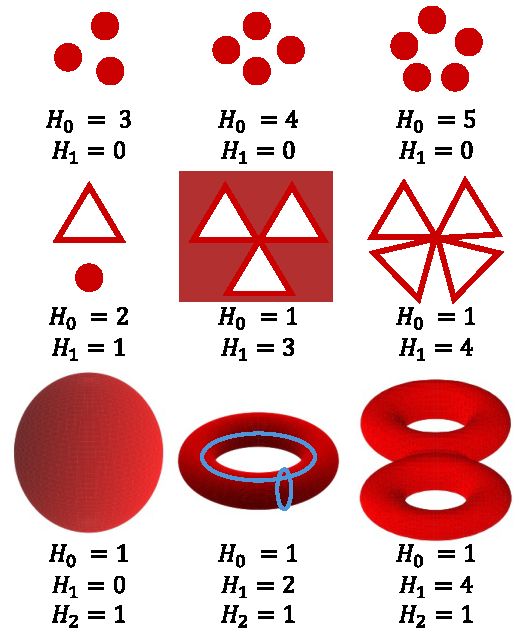
\includegraphics[width=\linewidth]{figures/topoexam.pdf}
        \caption{\textbf{Toy examples for homology.} We present the ranks of the homology groups of various topological spaces, i.e., for $\h_0(\X)=\BZ^k$ we write only $\h_0=k$ for simplicity, representing the count of the $k$-dimensional holes in $\X$.  \label{fig:homology}}    
\vspace{-.2in}
\end{wrapfigure}


To make the concept of homology groups more accessible, we will offer a simplified and visual explanation. 
We denote homology groups by $ \h_k(\X) $, where $ \X $ represents the space under consideration, and $ k $ indicates the dimension being analyzed. Independent $k$-holes are generators for the homology group $\h_k(\X)$. Therefore, the rank of $ \h_k(\X) $ indicates the number of $ k $-dimensional \textquote{holes} present in the space $ \X $. These numbers are also called {\em Betti numbers} $\{\beta_k(\X)\}$. e.g., if $\h_2(\X)=\BZ^3$, then we say rank($\h_2(\X))=3$ , or $\beta_2(\X)=3$, meaning $\X$ has three $2$-holes.  Below, we will give some examples for dimensions $0,1$ and $2$ (See \Cref{fig:homology}).




 
    
\noindent $\bullet$ \textbf{$\h_0(\X)$:} $0$-dimensional homology represents the connected components in $\X$. If $\X$ has three components, then we say $\h_0(\X)=\BZ^3$ (or $\BZ_2^3$ if used $\BZ_2$-coefficients), and rank$(\h_0(\X))=\beta_0(\X)=3$.
    

    \smallskip

    
\noindent $\bullet$ \textbf{$\h_1(\X)$:} $1$-dimensional homology computes the non-contractible loops (holes) in $\X$.
    For example, a sphere $\s$ has no nontrivial loops, as any loop in the sphere bounds a disk \underline{in the sphere}, i.e., $\beta_1(\s)=0$.
    A torus $\T$ (hollow donut), on the other hand, has meridian and longitude circles (see Figure~\ref{fig:homology}), both being non-contractible loops, making the total $\beta_1(\T)=2$. On the other hand, a solid donut $\D$ would have only the longitude circle as noncontractible, $\beta_1(\D)=1$.


    \smallskip
    
\noindent $\bullet$ \textbf{$\h_2(\X)$:} $2$-dimensional homology group captures two-dimensional cavities (voids) in the space $\X$. To count these cavities, we utilize surfaces in the space which does not bound a $3$-dimensional domain in the space. For example, in the unit ball $\B$ in $\R^3$ (solid ball), any closed surface bounds a 3-dimensional domain within $\B$, and there are no cavities within it. Hence, we say rank$(\h_2(\B))=\beta_2(\B)=0$. Similarly, if one removes two disjoint smaller balls from $\B$, say $\B'$, we would have two different cavities, which can be represented by different spheres in $\X$, enclosing these balls. Then, we say $\beta_2(\B')=2$. In~\Cref{fig:homology}, the sphere, the torus, or the genus-$2$ surface have one $2$-dimesional cavities represented by themselves.
    
  

We conclude this section with an interesting fact. While we defined the Euler characteristic for simplicial complexes as the alternating sum of the number of $k$-simplices, there is an alternative way using Betti numbers. In particular, if $\Y$ is a topological space, the Euler characteristic is given by $\chi(\Y)=\sum_k(-1)^k\beta_k(\Y)$.
 

\subsubsection{Computation of Homology} \label{sec:homology2}
We now turn to a formal introduction. Homology is a mathematical operation whose inputs are topological spaces and outputs are groups. In particular, for a given space $\X$, $\h_k(\X)$ represents the $k^{th}$ homology group of $\X$, summarizing the $k$-dimensional non-collapsible submanifolds in $\X$, each representing different $(k+1)$-dimensional "cavity" of $\X$. We will call these "$k$-holes" by abusing notation. 

The concept of homology groups stems from the idea that a $(k+1)$-dimensional hole or cavity in $\X$ is detected by the presence of its $k$-dimensional boundary, which cannot be continuously contracted within $\X$. While this method might seem indirect—using boundaries to infer the existence of cavities—the difficulty arises from the need to identify what is \textit{missing} in $\X$. Here, a fundamental principle of topology comes into play: \textit{the boundary of a boundary is always empty}. If $\Omega$ is a $(k+1)$-dimensional domain in $\X$ with boundary $\s = \partial \Omega$, then the boundary of $\s$ is empty. i.e., $\partial(\partial \Omega) = \partial \s=\emptyset$ Hence, to identify cavities, we first find all $k$-dimensional submanifolds with no boundary in $\X$ ($k$-cycles). Then, by eliminating those that bound a domain in $\X$ ($k$-boundaries), we are left with the true cavities. This process forms the core idea behind homology computation.


To keep the exposition focused, we will describe only \textit{simplicial homology with $\mathbb{Z}_2$ coefficients}, the most common version used in TDA. For other homology settings, refer to~\cite{hatcher2002algebraic}. In particular, simplicial homology involves representing a given space $\mathcal{X}$ as a simplicial complex (a collection of simplices) and performing computations on these simplices. This approach allows us to discretize the problem by focusing on the $k$-dimensional "building blocks" of the topological space, such as vertices for $0$-dimension and edges for $1$-dimension. By considering $k$-submanifolds  (or $k$-subcomplexes) as unions of $k$-simplices, we can identify the special ones that correspond to true cavities in $\mathcal{X}$ by using computational tools. To formalize this concept, we now introduce the relevant mathematical notions.


\paragraph*{i. Representation of $k$-simplices} In a simplicial complex $\X$, we describe $k$-simplices by listing their vertices. For example, a $1$-simplex (an edge) $e$ with endpoints $v_2$ and $v_4$ is denoted as $e = [v_2, v_4]$. Similarly, a $2$-simplex (a triangle) $\tau$ with vertices $v_1$, $v_5$, and $v_7$ is written as $\tau = [v_1, v_5, v_7]$. Since we are using $\mathbb{Z}_2$ coefficients, the order of the vertices does not matter. However, in other versions, such as with $\mathbb{Z}$-coefficients, the order of the vertices would be significant. In general, a $k$-simplex $\Delta$ is represented by its $k+1$ vertices, i.e., $\Delta = [v_{i_0}, v_{i_1}, \dots, v_{i_k}]$. We will call a union of $k$-simplices \textit{a $k$-subcomplex of $\X$}. 

\paragraph*{ii. $k$-chains $\C_k(\X)$} To describe all $k$-dimensional subcomplexes (which correspond to all $k$-submanifolds, with or without boundary) within a simplicial complex $\X$, we define a group $\C_k(\X)$, known as the group of {\em $k$-chains}. Recall that any union of $k$-simplices forms a $k$-subcomplex. For instance, if the simplicial complex $\X$ consists of three edges $\{e_1, e_2, e_3\}$, then all possible $1$-subcomplexes are $\{e_1, e_2, e_3, e_1 \cup e_2, e_1 \cup e_3, e_2 \cup e_3, e_1 \cup e_2 \cup e_3\}$. We represent this collection using group elements, where each $1$-simplex acts as a generator. In particular, the union $e_1 \cup e_3$ is represented by $\sigma_1 = (1,0,1)$, while $e_1 \cup e_2$ is represented by $\sigma_2 = (1,1,0)$. Hence, we obtain the group $\C_1(\X) = \BZ_2^3$, where $0$ element corresponds to the empty set. The group operation is addition, and since $1+1=0$ in $\BZ_2$, we have $\sigma_1 + \sigma_2 = (1,0,1) + (1,1,0) = (0,1,1)$, corresponding to the union $e_2 \cup e_3$. Similarly, if $\X$ contains $m$ $k$-simplices $\{\Delta_1, \Delta_2, \dots, \Delta_m\}$, then $\C_k(\X) = \BZ_2^m$, where a group element like $(1,0,1,\dots,1)$ represents the $k$-subcomplex $\Delta_1 \cup \Delta_3 \cup \Delta_m$ within $\X$.



\paragraph*{iii. Boundary operator $\partial_k$} To identify $k$-holes in a simplicial complex, we must first identify $k$-subcomplexes that have no boundary. This is accomplished by defining a boundary operator $\partial_k: \mathcal{C}_k(\X) \to \mathcal{C}_{k-1}(\X)$, which maps $k$-chains to their $(k-1)$-dimensional boundaries. In particular, $\partial_k$ maps each $k$-simplex to its boundary. For example, if we have a $1$-simplex (edge) $e = [v_0, v_1]$, then $\partial_1[e] = v_0 + v_1 \in \C_0(\X)$, representing the boundary of the edge as the union of its end vertices $\{v_0\} \cup \{v_1\}$. Similarly, for a $2$-simplex (triangle) $\tau = [v_0, v_1, v_2]$, the boundary is given by $\partial_2\tau = [v_0, v_1] + [v_1, v_2] + [v_2, v_0] \in \C_1(\X)$, representing the boundary of the triangle as the union $[v_0, v_1] \cup [v_1, v_2] \cup [v_2, v_0]$. 
To define $\partial_k$ for general $k$-chains, we sum the boundaries of each $k$-simplex within the chain. For instance, if $\sigma = \Delta_1 + \Delta_3 + \Delta_7$ is a $k$-chain, then $\partial_k\sigma = \partial_k\Delta_1 + \partial_k\Delta_3 + \partial_k\Delta_7$. 
A $k$-chain $\sigma$ is said to have \textit{no boundary} if $\partial_k\sigma = 0$. In other words, a $k$-subcomplex with no boundary in $\X$ must map to $0$ under the boundary operator.

The boundary operator $\partial_k: \mathcal{C}_k(\X) \to \mathcal{C}_{k-1}(\X)$ is a linear operator and can be represented as a matrix. For example, if $\mathcal{C}_k(\X) = \mathbb{Z}_2^n$ and $\mathcal{C}_{k-1}(\X) = \mathbb{Z}_2^m$, then $\partial_k$ can be written as an $m \times n$ matrix $\mathbf{A}$, with each column $\mathbf{A}_i$ corresponds to $\partial_k \Delta_i$, where $\Delta_i$ is a $k$-simplex in $\X$. In \Cref{fig:matrix1}, we give an explicit example of a matrix representation of a boundary operator the simplicial complex in \Cref{fig:toy1}.

\begin{wrapfigure}{r}{0.2\linewidth}
\vspace{-.15in}
    \centering
    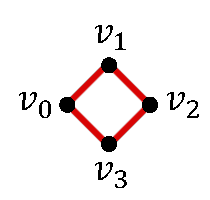
\includegraphics[width=\linewidth]{figures/toy1.pdf}
        \caption{\textbf{Toy example for homology.}   \label{fig:toy1}}    
\vspace{-.15in}
\end{wrapfigure}
\paragraph*{iv. $k$-cycles $\Z_k(\X)$} We define a special subgroup $\Z_k(\X)$, named \textit{$k$-cycles}, within $\C_k(\X)$ for $k$-subcomplexes that have no boundary. As previously mentioned, a $k$-subcomplex with no boundary in $\X$ must map to zero under the boundary operator. Hence, we define the subgroup $\Z_k(\X) = \ker \, \partial_k$, which includes all $k$-chains that map to zero.  Recall that $1$-chains with no boundary correspond to loops, while 2-chains with no boundary correspond to closed surfaces, like a sphere or torus.

For example, consider a square-shaped simplicial complex $\X$ (\Cref{fig:toy1}) with four vertices $\{v_0,v_1,v_2,v_3\}$ and four edges $\{e_1,e_2,e_3,e_4\}$  where $e_1=[v_0,v_1],e_2=[v_1,v_2],e_3=[v_2,v_3]$ and $e_4=[v_3,v_0]$. In this case, $\C_1(\X)=\BZ_2^4$ and $\C_0(\X)=\BZ_2^4$. Suppose $\sigma_1=e_1+e_2$; then $\partial_1\sigma_1= (v_0+v_1)+(v_1+v_2)=v_0+v_2$, meaning that $\sigma_1$ represents a 1-subcomplex with a boundary. However, if $\sigma_2=e_1+e_2+e_3+e_4$, then $\partial_1\sigma_2= (v_0+v_1)+(v_1+v_2)+(v_2+v_3)+(v_3+v_0)=2(v_0+v_1+v_2+v_3)=0$, indicating that $\sigma_2$ represents a 1-subcomplex with no boundary. Notice that $\sigma_2$ corresponds to a complete loop in $\X$. See \Cref{ex:toy1} for more details.

\begin{wrapfigure}{r}{1.3in}
\vspace{-.15in}
\footnotesize
$\partial_1 = 
\begin{array}{c}
\partial e_1 \ \partial e_2 \ \partial e_3 \ \partial e_4  \\
\begin{pmatrix}
1 & 0 & 0 & 1 \\ % v_0
1 & 1 & 0 & 0 \\ % v_1
0 & 1 & 1 & 0 \\ % v_2
0 & 0 & 1 & 1 % v_3
\end{pmatrix}
\end{array}
\textcolor{red}{
\begin{array}{c}
\ \\
v_0 \\
v_1 \\
v_2 \\
v_3
\end{array}}$
\caption{\footnotesize $\partial_1:\C_1(\X)\to\C_0(\X)$ is represented as a $4\times 4$ binary matrix. Columns represent the edges in $\C_1(\X)$, and rows correspond to the vertices in $\C_0(\X)$. For example,  $\partial e_3= v_2+v_3$ can be read from the third column \label{fig:matrix1}}
\vspace{-.2in}
\end{wrapfigure}


We can also describe the boundary map $\partial_1: \C_1(\X) \to \C_0(\X)$ as a $4 \times 4$ matrix, as shown in \Cref{fig:matrix1}. It is clear that the only element in $\C_1(\X)$ that maps to $(0,0,0,0) \in \C_0(\X)$ is $(1,1,1,1)$, which corresponds to the loop $\sigma_2$. This means $\X$ has only one $1$-cycle, which is $\sigma_2$. Then, $\Z_k(\X)$ is the subgroup of $\C_k(\X)$ generated by the single element $(1,1,1,1)$. If you are unfamiliar with group theory, you can think of $\C_1(\X)$ as a four-dimensional vector space, where $\Z_1(\X)$ is a one-dimensional subspace generated by the vector $(1,1,1,1)$.


\paragraph*{v. $k$-boundaries $\B_k(\X)$} While we identified all $k$-subcomplexes with no boundary, none correspond to true cavities. We must eliminate the ones that bounds a domain in $\X$. To find them, we use again the boundary operator. As $\C_{k+1}(\X)$ represents all $(k+1)$-subcomplexes in $\X$, then the image of $\partial_{k+1}$, i.e., $\B_k(\X) = \partial_{k+1}\mathcal{C}_{k+1}(\X) \subset \mathcal{C}_k(\X)$, represents the ones which bounds a $(k+1)$-domain in $\X$. We call an element in $\B_k(\X)$ a \textit{$k$-boundary}. Recall that $\partial_k(\partial_{k+1} \sigma)=0$ from earlier discussion. This means for any $k$-boundary $\varphi=\partial_{k+1} \sigma$ in $\B_k(\X)$, $\partial_k\varphi=0$. Therefore, we have $\B_k(\X)\subset\Z_k(\X)$. For example, if $\X$ is a simplicial complex formed by only one $2$-simplex $\tau$ with vertices $\{v_0,v_1,v_2\}$, then $\B_1(\X)$ would be a subgroup in $\C_1(\X)$, generated by $\partial_2 \tau=\sigma=(1,1,1)$ while $\Z_1(\X)$ would be the same group, i.e., $\Z_1(\X)=\B_1(\X)$. This means there is only one loop $\sigma$ in $\X$ but it does not represent a hole in $\X$ as it is filled by $\tau$, i.e., $\sigma=\partial \tau$.

\paragraph*{ vi. Homology group $\h_k(\X)$} Now we are ready to define homology. Notice that with the boundary operator, we obtained the following sequence of groups and maps. We can consider these as vector spaces and linear maps. For each $k$, $k$-chains $\C_k(\X)$ represent all $k$-subcomplexes in $\X$, $k$-cycles $\Z_k(\X)\subset \C_k(\X)$ represent $k$-subcomplexes with no boundary, and finally, $\B_k(\X)\subset \Z_k(\X)$ represent the $k$-subcomplexes which bounds a $(k+1)$-domain in $\X$.

\[
\begin{tikzcd}
\cdots \arrow[r, "\partial_{k+2}"] & \C_{k+1}(\X) \arrow[r, "\partial_{k+1}"] & \C_k(\X) \arrow[r, "\partial_k"] & \C_{k-1}(\X) \arrow[r, "\partial_{k-1}"] & \cdots \arrow[r, "\partial_1"] & \C_0(\X)\arrow[r] & 0
\end{tikzcd}
\]


 
Now, to identify $k$-holes (true cavities), we consider all $k$-cycles in $\X$ ($\Z_k(\X)$), which potentially represent a cavity of $\X$, and, among them, eliminate all $k$-boundaries in $\X$ ($\B_k(\X)$), as they represent the "fake" cavities. Hence, we define $k^{th}$ homology group as the quotient group $$\h_k(\X) = \Z_k(\X)/\B_k(\X) = \text{ker}(\partial_k)/\text{image}(\partial_{k+1})$$
In terms of the sequence above, this quotient $\h_k(\X) = \Z_k(\X)/\B_k(\X)$  effectively counts the $k$-dimensional cycles that correspond to actual holes or cavities in $\X$, not those that are merely boundaries of higher-dimensional regions. From a computational perspective, with this formulation, we only need to compute the kernels and images of a sequence of linear maps $\{\partial_k\}$ (binary matrices) to compute homology. 


\begin{wrapfigure}{r}{0.2\linewidth}
\vspace{-.2in}
    \centering
    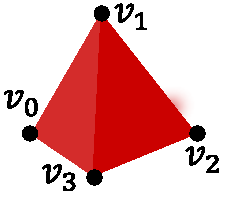
\includegraphics[width=\linewidth]{figures/toy2.pdf}
        \caption{\textbf{Toy example \ref{ex:toy2} for homology.}   \label{fig:toy2}}  
        \vspace{-.15in}
\end{wrapfigure}
To clarify these notions, we give two toy examples for explicit computation of homology.

\begin{example} \label{ex:toy1} Consider the example in \Cref{fig:toy1} where $\X$ is a square-shaped simplicial complex with four vertices $\{v_0, v_1, v_2, v_3\}$ and four edges. For $k \geq 2$, $\C_k(\X) = \{0\}$ since there are no $k$-simplices in $\X$. Both $\C_1(\X)$ and $\C_0(\X)$ are isomorphic to $\BZ_2^4$, as discussed earlier ($k$-cycles above). The group $\Z_1(\X)$ has only one generator, the sum of all edges. Since $\C_2(\X) = \{0\}$, we have $\B_1(\X) = \{0\}$ because $\B_1(\X) = \partial_2 \C_2(\X)$. Therefore, $\h_1(\X) = \Z_1(\X)/\B_1(\X) = \BZ_2/\{0\} = \BZ_2$, meaning that $\h_1(\X)$ has rank 1, corresponding to the entire square loop. The boundary map $\partial_1$ is given in~\Cref{fig:matrix1}.


For $\h_0(\X)$, we need to determine $\Z_0(\X)$ and $\B_0(\X)$. Since $\partial_0$ sends everything to 0, $\Z_0(\X) = \C_0(\X) = \BZ_2^4$. The group $\B_0(\X) = \partial_1 \C_1(\X)$ is generated by the boundaries of the edges: $(v_0 + v_1), (v_1 + v_2), (v_2 + v_3), (v_3 + v_0)$. However, these boundaries are not linearly independent because $v_3 + v_0$ is the sum of the other three boundaries. Thus, $\B_0(\X) \simeq \BZ_2^3$. Consequently, $\h_0(\X) = \Z_0(\X)/\B_0(\X) = \BZ_2^4/\BZ_2^3 = \BZ_2$. Recall that the rank of $\h_0(\X)$ represents the number of connected components and the fact that $\operatorname{rank}(\h_0(\X)) = 1$ confirms that there is only one connected component.  
\end{example}


\begin{wrapfigure}{r}{3.2in}
\vspace{-.1in}
\footnotesize
$\partial_2 = 
\begin{array}{c}
\partial \tau_1\ \partial \tau_2 \ \partial \tau_3 \ \partial \tau_4 \\ % Row of 'b's
\begin{pmatrix}
% t_1 t_2 t_3 t_4
1 & 0 & 1 & 0 \\ % e_1
1 & 1 & 0 & 0 \\ % e_2
0 & 1 & 0 & 1 \\ % e_3
0 & 0 & 1 & 1\\ % e_4
1 & 0 & 0 & 1 \\ % e_5
0 & 1 & 1 & 0   %e_6
\end{pmatrix} 
\end{array}
\textcolor{red}{
\begin{array}{c}
\ \\
e_1 \\
e_2 \\
e_3 \\
e_4 \\
e_5 \\
e_6
\end{array}}$ \ 
$\partial_1 = 
\begin{array}{c}
\partial e_1 \ \partial e_2 \ \partial e_3 \ \partial e_4 \ \partial e_5 \ \partial e_6 \\
\begin{pmatrix}
% e_1 e_2 e_3 e_4 e_5 e_6
1 & 0 & 0 & 1 & 1& 0 \\ % v_0
1 & 1 & 0 & 0 & 0 & 1 \\ % v_1
0 & 1 & 1 & 0 & 1 & 0\\ % v_2
0 & 0 & 1 & 1 & 0 & 1\\ % v_3
\end{pmatrix} 
\end{array}
\textcolor{red}{
\begin{array}{c}
\ \\
v_0 \\
v_1 \\
v_2 \\
v_3
\end{array}}$
\caption{\footnotesize {\bf Boundary maps for Ex. \ref{ex:toy2}.} The boundary map $\partial_2:\C_2(\X)\to\C_1(\X)$ is represented as a $6\times 4$ binary matrix (left). The top of each column corresponds to the $2$-simplex in $\C_2(\X)$ whose image is represented by that column, while each row's corresponding edge is given next to the column. For example, the boundary of $2$-simplex $\tau_2$, $\partial\tau_2= e_2+e_3+e_6$ by reading the second column in $\partial_2$ matrix. The boundary map $\partial_1:\C_1(\X)\to\C_0(\X)$ is similar (right). \label{fig:matrix2}}
\vspace{-.2in}
\end{wrapfigure}
Second example is in one dimension higher.

\begin{example} \label{ex:toy2} Consider the hollow tetrahedron $\X$ of \Cref{fig:toy2}, composed of four triangular faces: $\tau_1 = [v_0, v_1, v_2]$, $\tau_2 = [v_1, v_2, v_3]$, $\tau_3 = [v_0, v_1, v_3]$, and $\tau_4 = [v_0, v_2, v_3]$. The complex $\X$ contains four 2-simplices (triangles), six 1-simplices (edges), and four 0-simplices (vertices). Let $e_1=[v_0,v_1],e_2=[v_1,v_2], e_3=[v_2,v_3],e_4=[v_3,v_0], e_5=[v_0,v_2]$ and $e_6=[v_1,v_3]$. Therefore, we have $\C_2(\X) = \BZ_2^4$, $\C_1(\X) = \BZ_2^6$, and $\C_0(\X) = \BZ_2^4$. 



A straightforward computation shows that the kernel of $\partial_2$, denoted $\Z_2(\X)$, has a single generator: the sum of all the triangles, $\tau_1 + \tau_2 + \tau_3 + \tau_4$. Since there is no 3-simplex in $\X$, we find that $\B_2(\X) = \{0\}$, leading to $\h_2(\X) = \BZ_2$. This result aligns with the fact that rank$(\h_2(\X)) = 1$, indicating the presence of one cavity in $\X$, consistent with $\X$ being a hollow tetrahedron. We 
Furthermore, calculating $\Z_1(\X) = \BZ_2^3$ and $\B_1(\X) = \BZ_2$ shows that these cancel out, yielding $\h_1(\X) = \{0\}$. In other words, any loop in $\X$ is filled, so there is no $1$-hole in $\X$.
Similarly, following the same reasoning as in the example above, we obtain $\h_0(\X) = \BZ_2$ as expected.  
\end{example}






% To define homology, we take the set of all $k$-cycles and eliminate those that bound a $(k+1)$-dimensional region by quotienting them out. In other words, we define the $k$-th homology group as $\h_k(\X) = Z_k(\X)/B_k(\X)$. This quotient effectively counts the $k$-dimensional cycles that correspond to actual holes or cavities in $\X$, not those that are merely boundaries of higher-dimensional regions.

% At first glance, computing homology groups for topological spaces and their corresponding simplicial complexes might seem complex. However, in practice, any $k$-simplex can be uniquely defined by its $k+1$ vertices. For example, a $k$-simplex $\sigma^k$ can be represented as a list of its vertices, $\sigma^k = [v_{i_0}, v_{i_1}, \dots, v_{i_k}]$. Consequently, $\mathcal{C}_k(\X)$ is simply the collection of formal sums of these $k$-simplices. If there are $m_k$ $k$-simplices in $\X$, then each $k$-simplex serves as a generator for the $k$-chain group, making $\mathcal{C}_k(\X) = \BZ_2^{m_k}$, where $\BZ_2$ is the simplest group consisting of two elements (0 and 1). The number $m_k$ is called the rank of the group.

% In algebraic topology, the most common base group is $\BZ$, but for defining persistent homology properly, it is often necessary to choose a field as the base group. The common choice in TDA is $\BZ_2$~\cite{dey2022computational}. The boundary of each $k$-simplex is a collection of $(k-1)$-simplices. By using the image of each $k$-simplex, we define the boundary operator $\partial_k: \mathcal{C}_k(\X) \to \mathcal{C}_{k-1}(\X)$, which is a linear operator of dimension $m_{k-1} \times m_k$, where each column represents the boundary of one $k$-simplex in $\X$. From a computational perspective, this reduces the computation of homology to a problem in linear algebra: $\h_k(\X) = Z_k(\X)/B_k(\X) = \text{ker}(\partial_k)/\text{image}(\partial_{k+1})$.







%The next step is to identify all $k$-chains \textit{without boundaries} within $\mathcal{C}_k(\X)$. For instance, $1$-chains (which are unions of edges) without boundaries correspond to loops, while $2$-chains (unions of triangles) without boundaries correspond to surfaces like spheres or tori. To determine the boundaries of $k$-chains, we define a boundary operator $\partial_k: \mathcal{C}_k(\X) \to \mathcal{C}_{k-1}(\X)$, which maps $k$-chains to their $(k-1)$-dimensional boundaries. A $k$-chain $\Gamma$ is said to have no boundary if $\partial_k\Gamma = 0$. We then define a subset $\Z_k(\X) = \text{ker} \, \partial_k$, which represents all $k$-chains that map to zero. The elements of $\Z_k(\X)$ are referred to as $k$-cycles.




%Hence, we need an operation to determine whether a given $k$-subcomplex has a boundary or not. We define $\partial_k:\C_k(\X)\to\C_{k-1}(\X)$ from $k$-chains to 



% For example, if $\X$ has four $3$-simplices, say $\{\sigma_1, \sigma_2, \sigma_3, \sigma_4\}$, 
% %then $\C_3(\X)=\BZ^4=\{(n_1,n_2,n_3,n_4) \mid n_i\in \BZ\}$ where $(n_1,n_2,n_3,n_4)$ represents the $k$-chain $n_1\sigma_1+n_2\sigma_2+n_3\sigma_3+n_4\sigma_4$. Similarly, if we are using $\BZ_2$-coefficients, 
% then $\C_3(\X)=\BZ_2^4=\{(n_1,n_2,n_3,n_4) \mid n_i\in \BZ_2\}$ where $(n_1,n_2,n_3,n_4)$ represents the $k$-chain $n_1\sigma_1+n_2\sigma_2+n_3\sigma_3+n_4\sigma_4$. For example, $3$-chain $\Gamma_1=\sigma_1+\sigma_2\in \C_3(\X)$  represents the simplicial complex $\sigma_1\cup\sigma_2$, while $3$-chain $\Gamma_2=\sigma_1+\sigma_3+\sigma_4$ represents $\sigma_1\cup\sigma_3\cup\sigma_4$. With this idea, we can describe any union of $k$-dimensional simplices as a group element, $k$-chain.

%Simplicial homology is a method used to analyze a topological space $\X$ by representing it as a simplicial complex—a collection of simplices, such as vertices, edges, and higher-dimensional counterparts. By breaking the space down into these discrete pieces, we can focus on the $k$-dimensional elements (e.g., vertices for 0-dimension, edges for 1-dimension) to perform computational analysis.

% As mentioned above, to identify $k$-holes, we first need to find $k$-dimensional submanifolds {\em with no boundary}. For a $k$-dimensional simplicial complex $\K$ to form a $k$-manifold with no boundary, it must consist of a perfectly assembled collection of $k$-dimensional simplices. All the individual pieces must fit together seamlessly, without gaps or overlaps, ensuring that $S$ behaves like a continuous surface without breaks or edges (see~\Cref{fig:scsample} for examples). To describe the homology machinery 

% The definition of a homology group stems from the intuition that any $k+1$-dimensional hole or cavity in $\X$ is represented by its $k$-dimensional boundary. This might seem indirect to detect cavities in an object, however the main issue here is that as the cavity is not in $\X$, how can we detect something that does not belong in $\X$. At this point, we use a fundamental principle in topology: The boundary of a boundary is always empty. If $\Omega$ is $(k+1)$-dimensional domain in $\X$ and $\s=\partial \Omega$, then $\partial(\partial \Omega)=\partial \s=\emptyset$. Therefore, if we  first find all $k$-dimensional manifolds in $\X$ with no boundary, and eliminate all of them which bounds a domain in $\X$, then we are left with the cavities. This is the main idea behind homology computation. 

% For a $k$-dimensional simplicial complex $\K$ to form a $k$-manifold with no boundary, it must form a "perfect" collection of $k$-dimensional simplices, i.e., all the individual pieces must fit together seamlessly, without any gaps or excessive overlapping (see ~\Cref{fig:scsample} for examples). This seamless assembly is crucial because it ensures that $S$ behaves like a continuous surface without any breaks or edges.




%\textcolor{red}{The boundary $S$ within a space $\X$, it is often constructed from several $k$-dimensional simplices.} 
%The boundary $S$ of a $(k+1)$-dimensional manifold $\Omega$ within a space $\X$ is a $k$-dimensional manifold with no boundary ($\partial S = \emptyset$), which, in the context of simplicial homology, is often represented as a "perfect" collection of $k$-dimensional simplices. For $S$ to be considered a perfect union of these simplices to satisfy no boundary condition,  all the individual pieces must fit together seamlessly, without any gaps or excessive overlapping (see ~\Cref{fig:scsample} for examples). %This seamless assembly is crucial because it ensures that $S$ behaves like a continuous surface without any breaks or edges. In such cases, $S$ is said to have no boundary, which is denoted as $\partial S = \emptyset$. This condition signifies that when you explore the surface of $S$, you never encounter an abrupt stop at an edge, allowing $S$ to fully encapsulate the space it defines.} To understand this, consider what happens when you try to find the boundary of a shape. The boundary serves as the perimeter or outline of the shape. If one looks for the boundary of this outline, you'll find that it doesn't have its own outline—it simply marks the transition between the inside and the outside of the original shape. Since an perimeter or an outline does not have a further boundary, the result is always empty.



%\textcolor{blue}{A fundamental principle in topology states that the boundary of a boundary is always empty. This can be stated mathematically as $\partial (\partial S) = \emptyset$. To understand this, consider what happens when you try to find the boundary of a shape. The boundary serves as the perimeter or outline of the shape. If one looks for the boundary of this outline, you'll find that it doesn't have its own outline—it simply marks the transition between the inside and the outside of the original shape. Since an perimeter or an outline does not have a further boundary, the result is always empty.}

 

%\textN{Bu section sonuna dek ufak degisikliklere ugradi ama bunlari renk kodlamayla basa cikamadim}
 
% After this observation, homology is reduced to identifying the $k$-holes in the space as follows. First, we define a mathematical object, encoding all $k$-dimensional submanifolds (with or without boundary) in $\X$. $\mathcal{C}_k(\X)$, also called $k$-chains, is the group generated by all $k$-dimensional simplices in $\X$. While other coefficient rings, such as $\mathbb{Z}$, can be used, we focus exclusively on $\mathbb{Z}_2$-coefficients, the standard choice in TDA, to maintain clarity in our exposition. 
% %where a $k$-chain $\Delta\in \C_k(\X)$ is a formal sum of these $k$-simplices, While other coefficient rings (like $\BZ$) can be used, we only use $\BZ_2$-coefficients which is the common coefficient field used in TDA, to keep the exposition simple. 
% For example, if $\X$ has four $3$-simplices, say $\{\sigma_1, \sigma_2, \sigma_3, \sigma_4\}$, 
% %then $\C_3(\X)=\BZ^4=\{(n_1,n_2,n_3,n_4) \mid n_i\in \BZ\}$ where $(n_1,n_2,n_3,n_4)$ represents the $k$-chain $n_1\sigma_1+n_2\sigma_2+n_3\sigma_3+n_4\sigma_4$. Similarly, if we are using $\BZ_2$-coefficients, 
% then $\C_3(\X)=\BZ_2^4=\{(n_1,n_2,n_3,n_4) \mid n_i\in \BZ_2\}$ where $(n_1,n_2,n_3,n_4)$ represents the $k$-chain $n_1\sigma_1+n_2\sigma_2+n_3\sigma_3+n_4\sigma_4$. For example, $3$-chain $\Gamma_1=\sigma_1+\sigma_2\in \C_3(\X)$  represents the simplicial complex $\sigma_1\cup\sigma_2$, while $3$-chain $\Gamma_2=\sigma_1+\sigma_3+\sigma_4$ represents $\sigma_1\cup\sigma_3\cup\sigma_4$. With this idea, we can describe any union of $k$-dimensional simplices as a group element, $k$-chain.



%then the set of all cycles $Z_k(\X)$ is the kernel of this operator, i.e., $Z_k(\X) = \text{ker} \, \partial_k$, representing all $k$-chains that map to zero, meaning they have no boundary. 


%For obtain a $k$-chain with no boundary, it must be a "perfect" collection of $k$-dimensional simplices, i.e., all the individual pieces must fit together seamlessly, without any gaps or excessive overlapping (see ~\Cref{fig:scsample} for examples). This seamless assembly is crucial because it ensures that $S$ behaves like a continuous surface without any breaks or edges.



%These are $k$-chains that have no boundary themselves, meaning they represent closed loops, surfaces, or higher-dimensional analogs within $\X$. We call such $k$-chains $k$-cycles. In homology, the concept of a cycle extends beyond just loops. It encompasses higher-dimensional analogs of loops, such as closed surfaces (2-cycles), closed volumes (3-cycles), and so on. For instance, consider a union $S$ of $k$-simplices in $\X$. If the boundary $\partial S$ is not empty, then $S$ is a $k$-chain but not a $k$-cycle. If $\partial S = \emptyset$, meaning $S$ has no boundary, then it is a $k$-cycle. We denote the set of all $k$-cycles as $Z_k(\X) \subset \mathcal{C}_k(\X)$. Hence, $Z_k(\X)$ represents all the potential $k$-dimensional boundaries in $\X$.

% More formally, if $\partial_k: \mathcal{C}_k(\X) \to \mathcal{C}_{k-1}(\X)$ is the boundary operator that maps $k$-chains to their $(k-1)$-dimensional boundaries, then the set of all cycles $Z_k(\X)$ is the kernel of this operator, i.e., $Z_k(\X) = \text{ker} \, \partial_k$, representing all $k$-chains that map to zero, meaning they have no boundary.  



% Now, $\Z_k(\X)$ captures all potential $k$-chains with no boundaries, but not all of these are necessarily associated with a "hole" or "cavity" in $\X$. Some of these $k$-cycles might be the boundary of a $(k+1)$-dimensional region within $\X$. For example, the surface of a 3-dimensional ball is a 2-dimensional cycle, but it bounds a 3-dimensional volume, so it does not correspond to a true cavity. To identify true cavities, we need to filter out these boundaries that enclose a $(k+1)$-dimensional domain. We do this by considering the boundaries of all $(k+1)$-chains, denoted as $B_k(\X) = \partial_{k+1}\mathcal{C}_{k+1}(\X) \subset \mathcal{C}_k(\X)$. Since the boundary of a boundary is always empty, we have $B_k(\X) \subset Z_k(\X)$. We call any $k$-chain in $B_k(\X)$ a $k$-boundary. Thus, while $Z_k(\X)$ represents all $k$-cycles (potential boundaries of $(k+1)$-dimensional domains), $B_k(\X)$ represents those that actually bound such domains, meaning they are not associated with true cavities.